<<<<<<< Updated upstream
\documentclass[10pt,pdf,hyperref={unicode}]{beamer}

\mode<presentation>
{
\usetheme{boxes}
\beamertemplatenavigationsymbolsempty

\setbeamertemplate{footline}[page number]
\setbeamersize{text margin left=0.5em, text margin right=0.5em}
}

\usepackage[utf8]{inputenc}
\usepackage[english, russian]{babel}
\usepackage{bm}
\usepackage{multirow}
\usepackage{ragged2e}
\usepackage{indentfirst}
\usepackage{multicol}
\usepackage{subfig}
\usepackage{amsmath,amssymb}
\usepackage{enumerate}
\usepackage{mathtools}
\usepackage{comment}
\usepackage{multicol}

\usepackage[all]{xy}

\usepackage{tikz}
\usetikzlibrary{positioning,arrows}

\tikzstyle{name} = [parameters]
\definecolor{name}{rgb}{0.5,0.5,0.5}

\usepackage{caption}
\captionsetup{skip=0pt,belowskip=0pt}

\newtheorem{rustheorem}{Теорема}
\newtheorem{russtatement}{Утверждение}
\newtheorem{rusdefinition}{Определение}

% colors
\definecolor{darkgreen}{rgb}{0.0, 0.2, 0.13}
\definecolor{darkcyan}{rgb}{0.0, 0.55, 0.55}

\AtBeginEnvironment{figure}{\setcounter{subfigure}{0}}

\captionsetup[subfloat]{labelformat=empty}

%----------------------------------------------------------------------------------------------------------

\title[Пример слайдов по работе]{Пример слайдов по работе \\ курса}
\author{И.\,О.\,Фамилия}

\institute[]{Московский физико-технический институт}
\date[2022]{\small 10\;февраля\;2022\,г.}

%---------------------------------------------------------------------------------------------------------
\begin{document}

\begin{frame}
\titlepage
\end{frame}

%----------------------------------------------------------------------------------------------------------
\section{Слайд об исследованиях}
\begin{frame}{Слайд об исследованиях}
\bigskip
Исследуется проблема \ldots.
\begin{block}{Цель исследования~---}
предложить метод \ldots.
\end{block}
\begin{block}{Требуется предложить}
\justifying
\begin{enumerate}[1)]
\item метод \ldots,
\item метод \ldots,
\item метод \ldots.
\end{enumerate}
\end{block}
\begin{block}{Решение}
Для \ldots.
\end{block}
\end{frame}

%---------------------------------------------------------------------------------------------------------
\section{Постановка задачи \ldots}
\begin{frame}{Постановка задачи \ldots}
Заданы
\begin{enumerate}[1)]
    \item признаки \ldots,
    \item целевая переменная \ldots,
    \item \ldots.
\end{enumerate}

\ldots

\bigskip

Требуется выбрать модель \ldots из множества
\[
	\mathfrak{G} = \left\{\mathbf{g}| \mathbf{g}:\mathbb{R}^{n} \to \mathbb{Y}^\prime\right\}.
\]
Оптимизационная задача \ldots:
\[
	\mathbf{g} = \arg\min_{\mathbf{g} \in \mathfrak{G}} \mathcal{L}\bigr(\ldots\bigr),
\]
где $\mathcal{L}$~--- функция ошибки.

\bigskip
\footnotetext[1]{\textit{Lopez-Paz D., Bottou L., Scholkopf B., Vapnik V.} Unifying distillation and privileged information // ICLR, 2016.}
\footnotetext[2]{\textit{Hinton G., Vinyals O., Dean J.} Distilling the knowledge in a neural network // NIPS, 2015.}
\end{frame}

%----------------------------------------------------------------------------------------------------------
\section{Предложенный метод \ldots}
\begin{frame}{Предложенный метод \ldots}
~\\[-1mm]
Заданы
\begin{enumerate}[1)]
	\item \ldots,
	\item \ldots.
\end{enumerate}

\medskip
Параметрические семейства:
\[
\setlength\abovedisplayskip{0pt}
\mathfrak{F} = \left\{\mathbf{f}| \mathbf{f} = \text{softmax}\bigr(\mathbf{v}\bigr(\mathbf{x}\bigr)/T\bigr), \quad \mathbf{v}: \mathbb{R}^{n} \to \mathbb{R}^K \right\},
\]
\[
\mathfrak{G} = \left\{\mathbf{g}| \mathbf{g} = \text{softmax}\bigr(\mathbf{z}\bigr(\mathbf{x}\bigr)/T\bigr), \quad \mathbf{z}: \mathbb{R}^n \to \mathbb{R}^K \right\},
\]
где~\ldots.

\medskip
Функция ошибки
\[
\setlength\abovedisplayskip{0pt}
\begin{aligned}
   \mathcal{L}\bigr(\mathbf{g}\bigr) = &-\sum_{i=1}^{m}\underbrace{{\sum_{k=1}^{K}y^k_i\log\mathbf{g}\bigr(\mathbf{x}_i\bigr)\bigr|_{T=1}}}_{\text{исходная функция потерь}}- \sum_{i=1}^{m}\underbrace{{\sum_{k=1}^{K}\mathbf{f}\bigr(\mathbf{x}_i\bigr)\bigr|_{T=T_0}\log\mathbf{g}\bigr(\mathbf{x}_i\bigr)\bigr|_{T=T_0}}}_{\text{слагаемое дистилляции}},
\end{aligned}
\setlength\belowdisplayskip{0pt}
\]
где~\ldots.

Оптимальная модель выбирается из класса,
$\hat{\mathbf{g}} = \arg\min\limits_{\mathbf{g} \in \mathfrak{G}_{\text{cl}}} \mathcal{L}\bigr(\mathbf{g}\bigr).$
\end{frame}

%----------------------------------------------------------------------------------------------------------
\section{Анализ предложенного метода \ldots}
\begin{frame}{Анализ предложенного метода \ldots}
\justifying

На графике показана зависимость значения параметров$w_i$ в зависимости от параметра~$l_1$-регуляризации~$C$.
\begin{figure}[h!]
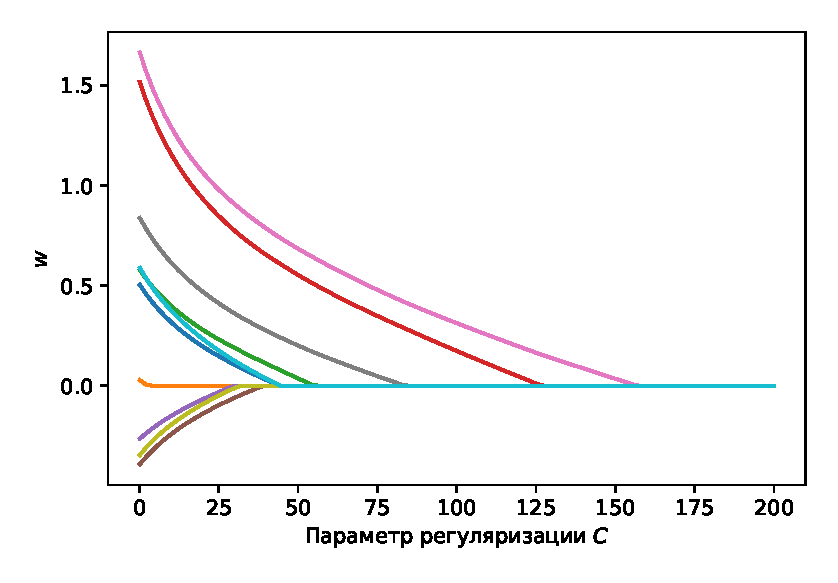
\includegraphics[width=0.45\textwidth]{../figures/log_reg_cs_exp.eps}
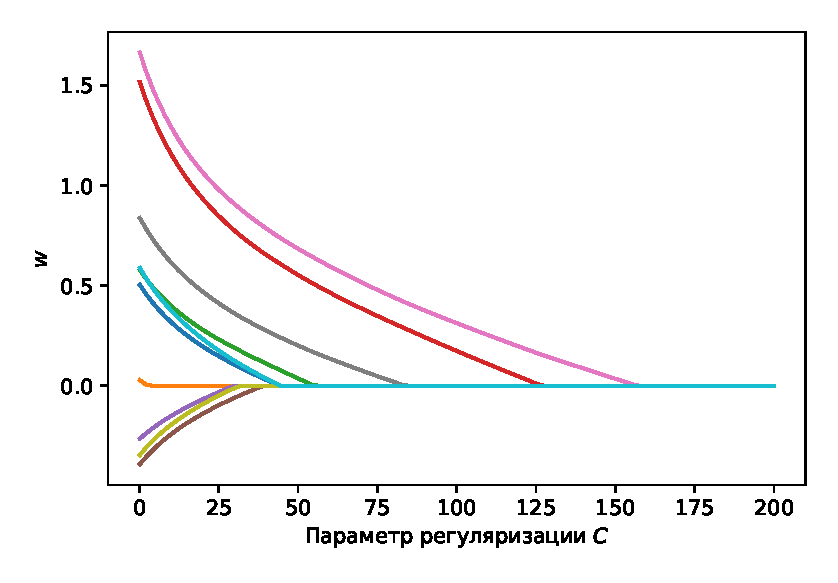
\includegraphics[width=0.45\textwidth]{../figures/log_reg_cs_exp.eps}
\end{figure}

С увеличением параметра регуляризации~$C$ число ненулевых параметров~$w_i$ уменьшается.

\end{frame}

%----------------------------------------------------------------------------------------------------------
\section{Выводы}
\begin{frame}{Выводы}
\justifying
	\begin{enumerate}
	\justifying
	    \item Предложен \ldots.
        \item Доказаны теоремы \ldots, 
        \begin{itemize}
            \item[---] \ldots,
            \item[---] \ldots.
        \end{itemize}
        \item Предложен метод \ldots
        \begin{itemize}
            \item[---] \ldots,
            \item[---] \ldots.
        \end{itemize}
        \item Предложены методы \ldots
        \begin{itemize}
            \item[---] \ldots,
            \item[---] \ldots.
        \end{itemize}
        \item Предложена вероятностная интерпретации \ldots.
	\end{enumerate}
\end{frame}
%----------------------------------------------------------------------------------------------------------

\end{document} 
=======
%\documentclass[c]{beamer}  % [t], [c], или [b] --- вертикальное выравнивание на слайдах (верх, центр, низ)
%\documentclass[handout]{beamer} % Раздаточный материал (на слайдах всё сразу)
\documentclass[10pt,pdf]{beamer} % Соотношение сторон
\usepackage[labelfont=bf]{caption}
\usepackage{subfig} % for subfigures
\usepackage{bm}
%\usetheme{Bergen}
\usetheme{Berlin}
%\usetheme{Warsaw}

%\useoutertheme{тема}
%\useinnertheme{тема} 

\setbeamercolor{background canvas}{bg=white}
\useinnertheme{circles}

%%% Работа с русским языком
\usepackage{cmap}					% поиск в PDF
\usepackage{mathtext} 				% русские буквы в формулах
\usepackage[T2A]{fontenc}			% кодировка
\usepackage[utf8]{inputenc}			% кодировка исходного текста
\usepackage[english,russian]{babel}	% локализация и переносы
\usepackage{graphicx}
\usepackage{geometry}
\usepackage{lipsum}
%% Beamer по-русски
\newtheorem{rtheorem}{Теорема}
\newtheorem{rproof}{Доказательство}
\newtheorem{rexample}{Пример}

%%% Дополнительная работа с математикой
\usepackage{amsmath,amsfonts,amssymb,amsthm,mathtools} % AMS
\usepackage{icomma} % "Умная" запятая: $0,2$ --- число, $0, 2$ --- перечисление

%% Номера формул
%\mathtoolsset{showonlyrefs=true} % Показывать номера только у тех формул, на которые есть \eqref{} в тексте.
%\usepackage{leqno} % Нумерация формул слева

%% Свои команды
\DeclareMathOperator{\sgn}{\mathop{sgn}}



%%% Работа с картинками
\usepackage{graphicx}  % Для вставки рисунков
\setlength\fboxsep{3pt} % Отступ рамки \fbox{} от рисунка
\setlength\fboxrule{1pt} % Толщина линий рамки \fbox{}
\usepackage{wrapfig} % Обтекание рисунков текстом

%%% Работа с таблицами
\usepackage{array,tabularx,tabulary,booktabs} % Дополнительная работа с таблицами
\usepackage{longtable}  % Длинные таблицы
\usepackage{multirow} % Слияние строк в таблице

%%% Программирование
\usepackage{etoolbox} % логические операторы

%%% Другие пакеты
\usepackage{lastpage} % Узнать, сколько всего страниц в документе.
\usepackage{soul} % Модификаторы начертания
\usepackage{csquotes} % Еще инструменты для ссылок
%\usepackage[style=authoryear,maxcitenames=2,backend=biber,sorting=nty]{biblatex}
\usepackage{multicol} % Несколько колонок

%%% Картинки
\usepackage{tikz} % Работа с графикой
\usepackage{pgfplots}
\usepackage{pgfplotstable}

\title{Предсказание показания фМРТ по видео, показанному человеку}
\author{Дорин Даниил}
\date{\today}
\institute[Московский физико-технический институт]{Московский физико-технический институт }

\setbeamercovered{transparent = 15}

\begin{document}

	\begin{frame}{}
		\maketitle
	\end{frame}

%%%%%%%%%%%%%%%%%%%%%%%%%%%%%%%%%%%%%%%%%%%%%%%%%%%%%%%%%%%%%%%%%%%%%%%%%%%%%%%%%%%%%%%%%%%
\begin{frame}{}

\begin{block}{Описание модели:}
\begin{equation}
	\label{basic_model}
	\bm{f}(\bm{x}_{k_m - \nu \cdot \Delta t}) = \bm{s}^m,
\end{equation}

	\[f_{ijk}(\bm{x}, \bm{W}_{ijk}) = \langle \bm{x}, \bm{W}_{ijk} \rangle,\]
\begin{enumerate}
    \item $\bm{s}^m \in \mathbb{R}^{40 \times 64 \times 64}$~--- тензор снимка фМРТ под номером $m$
    \item $\bm{x} = [x_1, \ldots, x_{d}]^{T}$~--- вектор признаков изображения, $d=2048$ 
    \item $\bm{W}_{ijk} = [w^{ijk}_1, \ldots, w^{ijk}_{d}]^{T}$~--- вектор весов элемента тензора $s_{ijk}$
\end{enumerate}
\end{block}

\begin{block}{Loss function:}
\begin{equation}
	\label{Loss}
	\mathcal{L}_{ijk}(\bm{W}_{ijk}, \Delta t) = \sum\limits_{m = 1}^{641 - \mu \cdot \Delta t} \big(f_{ijk}(\bm{x}_m, \bm{W}_{ijk}) - s^{m}_{ijk}\big)^2.
\end{equation}
\end{block}
\end{frame}

\begin{frame}{}
\begin{figure}[h!]
    \centering
    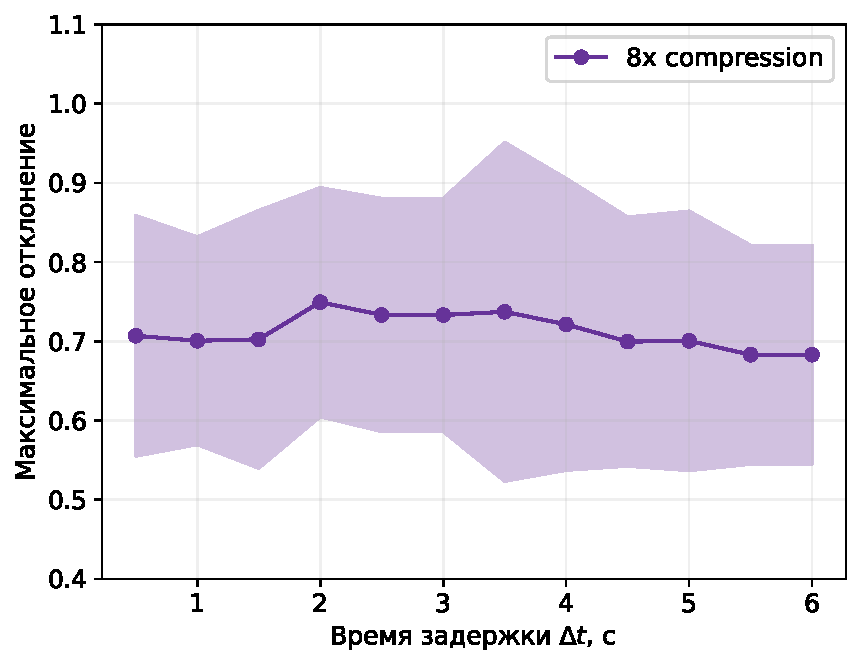
\includegraphics[scale = 0.34]{subs_deviation_dt.pdf}
    \label{MSE_dt}
\end{figure}
\begin{figure}[h!]
    \centering
    \subfloat[Оригинальный]{\label{fig:3-orig}{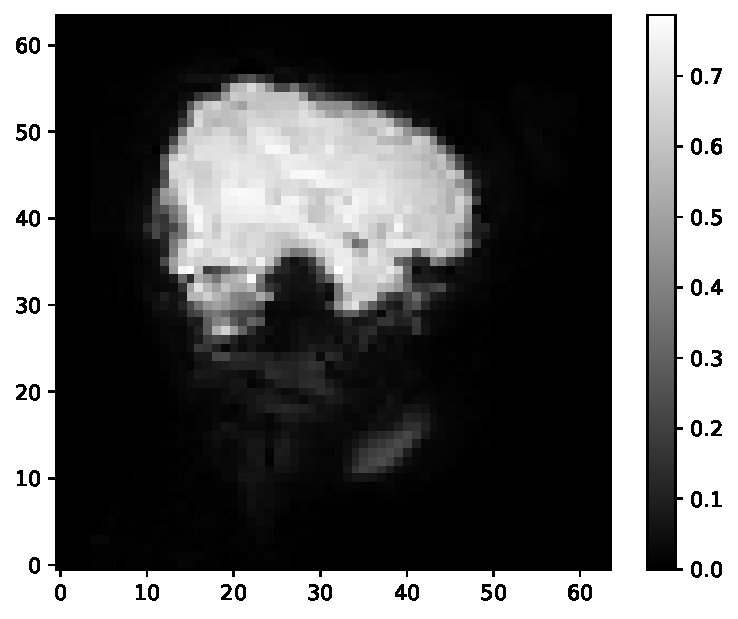
\includegraphics[width=0.3\textwidth]{sub-4-04-1-10-_-_-orig.pdf}}}
    \hfill
    \subfloat[Предсказанный]{\label{fig:3-pred}{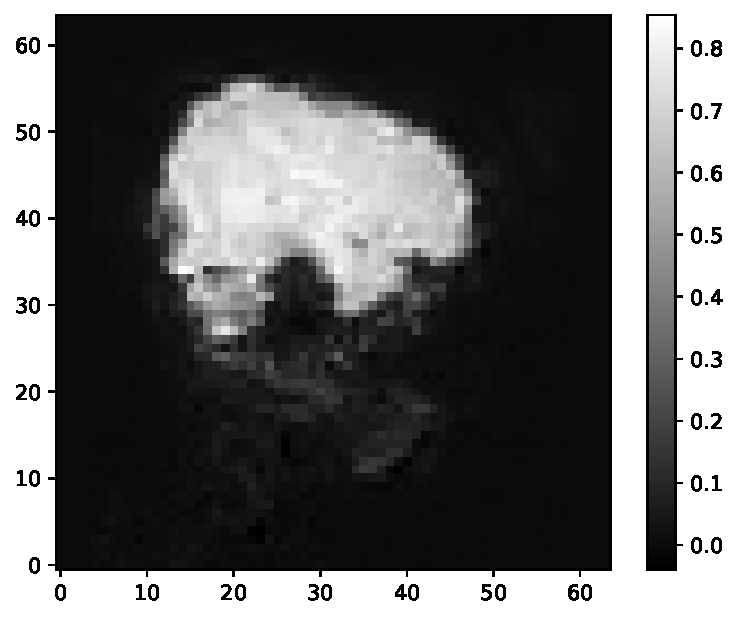
\includegraphics[width=0.3\textwidth]{sub-4-04-1-10-_-_-pred.pdf}}}
    \hfill
    \subfloat[Разность]{\label{fig:3-delta}{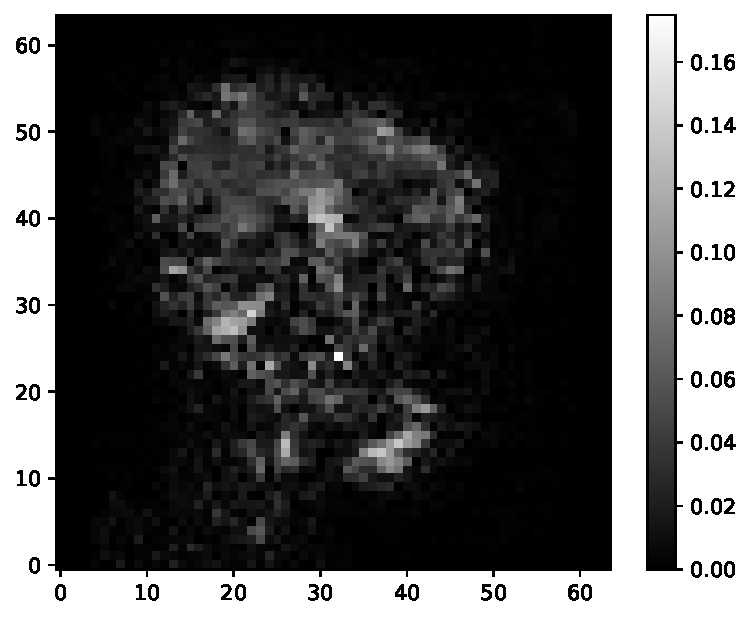
\includegraphics[width=0.3\textwidth]{sub-4-04-1-10-_-_-delta.pdf}}}
  
    \label{fig:3}
\end{figure}
\end{frame}

\end{document}
>>>>>>> Stashed changes
